% =====================================================================================
% Fashion-MNIST: Handcrafted vs Learned Features -- Capstone Phase 2 Report (IEEE conference format)
%
% COMPILE (Overleaf):
%   1. New project -> paste this file as main.tex.
%   2. Upload these 5 PNGs from results/figures/ next to main.tex (same folder, not a subfolder):
%        cnn_training_curves.png                      cnn_recall_vs_classical.png
%        errors_confusion_cnn3_images.png             errors_misclassified_rbf_svm_hog_shirt_vs_t-shirt_top.png
%        errors_misclassified_cnn3_images_shirt_vs_t-shirt_top.png
%   3. Compiler: pdfLaTeX. IEEEtran ships with Overleaf.
%
% Every number comes from results/summary_all.csv, results/metrics/*.json, results/training/*.csv and the saved test
% predictions. Confidence intervals (Wilson, 95%) and McNemar tests were computed from those files; no model was re-run
% on the test set.
% =====================================================================================
\documentclass[conference]{IEEEtran}
\IEEEoverridecommandlockouts

\usepackage[utf8]{inputenc}
\usepackage[T1]{fontenc}
\usepackage[final,expansion=false]{microtype}
\usepackage{graphicx}
\usepackage{booktabs}
\usepackage{multirow}
\usepackage{array}
\usepackage{threeparttable}
\usepackage{amsmath,amssymb}
\usepackage{xcolor}
\usepackage{tikz}
\usetikzlibrary{positioning,arrows.meta,fit,backgrounds}
\usepackage{url}
\usepackage{cite}
\usepackage[hidelinks]{hyperref}
\usepackage[capitalise,nameinlink]{cleveref}

% ---- consistent notation -----------------------------------------------------------
\newcommand{\pp}{\,pp}                       % percentage points
\newcommand{\RQ}[1]{\textbf{RQ#1}}
\newcommand{\best}[1]{\textbf{#1}}
\newcommand{\arrowc}{\,$\rightarrow$\,}

\crefname{table}{Table}{Tables}
\crefname{figure}{Fig.}{Figs.}
\crefname{section}{Section}{Sections}
\crefname{equation}{Eq.}{Eqs.}

\begin{document}

\title{Do Learned Features Resolve Fine-Grained Garment Confusions?\\[2pt]
\large A Controlled Comparison of Small Convolutional Networks and\\Handcrafted-Feature Classifiers on Fashion-MNIST}

\author{
\IEEEauthorblockN{Tanmay Singh, Anand Mishra, Rajdeep Sanyal, Rajat Srivastav, Omved Nagre}
\IEEEauthorblockA{Newton School of Technology, Rishihood University\\
Advanced Machine Learning and Deep Learning --- Capstone Project, Phase~2}
}

\maketitle

% =====================================================================================
\begin{abstract}
Convolutional neural networks (CNNs) are widely assumed to beat handcrafted image features, but the size of that
advantage, and where it comes from, is rarely measured under a protocol strict enough to trust. In earlier work we built a
leak-free classical baseline on Fashion-MNIST, whose best model, an RBF support vector machine on Histogram of Oriented
Gradients (HOG) features, reached 91.08\% test accuracy and, like every classical model, confused Shirt with
T-shirt/top, Pullover and Coat. We stated two hypotheses before training any network: a small CNN would exceed that
accuracy, and it would do so chiefly by resolving the upper-body garment confusions. We train two- and three-block CNNs
with pooling, dropout and early stopping on the \emph{identical} split, select between them on validation only, and score
them once with the \emph{identical} evaluation code. The selected three-block network reaches 92.09\% test accuracy
(95\% CI 91.54--92.60\%) and 0.9208 macro-F1, 101 fewer errors than the SVM (McNemar $p=2.2\times10^{-4}$), while
predicting ${\sim}300\times$ faster from a model ${\sim}377\times$ smaller. The first hypothesis holds; the second fails
in an instructive way. Shirt recall is unchanged (75.1\% vs.\ 75.2\%, $p=1.0$): the two models trade shirts rather than
fix them, the CNN's gains are spread over the other tops, footwear and trousers, and the four upper-body classes hold a
\emph{larger} share of its residual errors. Of the 475 images both models misclassify, 398 receive the same wrong label, and visual inspection
reveals collarless and sleeveless garments labeled Shirt. We argue that this residual error reflects the information
content of $28\times28$ images and their labels rather than the choice of representation.
\end{abstract}

\begin{IEEEkeywords}
Convolutional neural networks, Fashion-MNIST, handcrafted features, HOG, support vector machines, early stopping,
dropout, McNemar test, error analysis, label ambiguity
\end{IEEEkeywords}

% =====================================================================================
\section{Introduction}
\label{sec:intro}
Representation learning is the central promise of deep learning: instead of an engineer deciding which image
statistics matter, a network learns its own features from data~\cite{lecun2015deep}. For natural images the promise has
been kept spectacularly~\cite{krizhevsky2012imagenet,simonyan2015very,he2016deep}. Yet on small, low-resolution
benchmarks the gap between learned and handcrafted features is narrower, and claims about it are often weakened by
protocol choices---test sets reused for tuning, models compared after training on different amounts of data, or
single-number comparisons without uncertainty~\cite{kaufman2012leakage,cawley2010overfitting,bouthillier2021accounting}.

Phase~1 of this project~\cite{phase1report} established a strong, leak-free classical baseline on
Fashion-MNIST~\cite{xiao2017fashion}: twelve experiments over five classifiers and two representations, with every
decision taken on a fixed validation split and every test-set access logged. The best model, an RBF SVM on HOG
features~\cite{dalal2005histograms,cortes1995support}, reached 91.08\% test accuracy. Its errors were highly structured:
Shirt was the hardest class for all ten trained models, and confusions among \{T-shirt/top, Pullover, Coat, Shirt\} made up
56--66\% of every model's errors. Phase~1 closed with an explicit, falsifiable prediction, which we restate as two
hypotheses:
\begin{itemize}
  \item \textbf{H1 (accuracy).} A small CNN trained under the same protocol exceeds 91.08\% test accuracy.
  \item \textbf{H2 (mechanism).} Its gain comes \emph{chiefly} from resolving confusions within the four upper-body
        garments, because learned local filters capture the collars, buttons and cuffs that fixed edge histograms miss.
\end{itemize}
H2 is the more interesting claim: it predicts not only \emph{that} learned features help but \emph{where}. We test both
through four research questions that extend Phase~1's RQ1--RQ4:
\begin{itemize}
  \item \RQ{5}: Does a small CNN beat the best classical model on accuracy and macro-F1?
  \item \RQ{6}: Does it reduce the Shirt / T-shirt / Pullover / Coat confusion?
  \item \RQ{7}: Does a third convolutional block help?
  \item \RQ{8}: What does the CNN cost in parameters, model size and inference time?
\end{itemize}

\textbf{Contributions.}
(i)~A controlled comparison in which the CNN and the classical models share the split, the test set, the metrics and
the evaluation code, so differences are attributable to the representation and classifier alone;
(ii)~a depth ablation with a validation-only selection rule fixed before training, reported with its run-to-run
uncertainty;
(iii)~paired significance tests and an image-level agreement analysis showing that the CNN's gain is real but does not
arise where the prior hypothesis predicted; and
(iv)~evidence that the residual error is dominated by images whose labels are ambiguous at $28\times28$, a ceiling that
neither representation crosses.

\textbf{Summary of findings.} H1 is supported: 92.09\% vs.\ 91.08\%, significant at $p=2.2\times10^{-4}$. H2 is
not: Shirt recall is unchanged and the CNN's improvement is spread across T-shirt/top, Pullover, Coat and the footwear and
trouser classes. The three-block network is chosen on validation, but its advantage over the two-block network is not
statistically distinguishable from zero; what depth reliably buys is a 43\% smaller model.

% =====================================================================================
\section{Related Work}
\label{sec:related}
\textbf{From receptive fields to CNNs.} Hubel and Wiesel showed that neurons in the cat visual cortex respond to
oriented edges within small receptive fields and are organized hierarchically~\cite{hubel1962receptive}. Fukushima's
Neocognitron turned this into a model of alternating feature-extracting and pooling layers~\cite{fukushima1980neocognitron}.
LeCun~\emph{et al.}\ trained such architectures end to end with backpropagation~\cite{rumelhart1986learning}, first for
zip codes~\cite{lecun1989backpropagation} and then in LeNet-5 for document recognition~\cite{lecun1998gradient}; our
networks are direct descendants of LeNet. AlexNet~\cite{krizhevsky2012imagenet} combined depth, ReLU
activations~\cite{nair2010rectified}, dropout and GPU training to win ImageNet by a wide margin, and later work showed that
depth with small $3\times3$ filters~\cite{simonyan2015very} and residual connections~\cite{he2016deep} keep improving
accuracy. A textbook treatment of the building blocks we use is given by Goodfellow~\emph{et al.}~\cite{goodfellow2016deep}.

\textbf{Handcrafted vs.\ learned features.} HOG~\cite{dalal2005histograms} summarizes local gradient orientations in
normalized cell histograms and was the dominant descriptor for object detection before deep learning. Zeiler and
Fergus~\cite{zeiler2014visualizing} showed that the first layers of a trained CNN learn edge and color-blob detectors
resembling such descriptors, while deeper layers respond to object parts. Razavian~\emph{et al.}~\cite{razavian2014cnn}
found that generic CNN activations fed to a linear SVM outperform tuned handcrafted pipelines across many recognition
tasks. Our comparison holds the data and protocol fixed and asks the narrower question of \emph{which errors} a small
learned representation removes.

\textbf{Regularization and optimization.} Dropout randomly removes units during training, preventing co-adaptation and
approximating an ensemble~\cite{srivastava2014dropout}. Early stopping treats the number of training epochs as a
hyperparameter chosen on held-out data~\cite{prechelt1998early}. Adam adapts per-parameter step sizes from running moment
estimates~\cite{kingma2015adam}. Batch normalization~\cite{ioffe2015batch} and data augmentation are deliberately
excluded here, as they are not part of the specified architecture.

\textbf{Fashion-MNIST.} Xiao~\emph{et al.}~\cite{xiao2017fashion} released Fashion-MNIST as a harder drop-in replacement
for MNIST and reported scikit-learn baselines up to 89.7\%. Wide residual networks~\cite{zagoruyko2016wide} trained with
random-erasing augmentation reach about 96\%~\cite{zhong2020random}, using orders of magnitude more parameters than our
networks. Our goal is not state-of-the-art accuracy but a controlled measurement of what a small, specified CNN changes.

\textbf{Rigorous evaluation.} Test-set reuse inflates reported scores~\cite{kaufman2012leakage}, and selecting the best of
several configurations biases the winning validation score~\cite{cawley2010overfitting}. Dietterich recommends
McNemar's test~\cite{mcnemar1947note} for comparing two classifiers on one test set~\cite{dietterich1998approximate}, and
Bouthillier~\emph{et al.}~\cite{bouthillier2021accounting} show that seed-dependent variation can rival the differences
being reported. Northcutt~\emph{et al.}~\cite{northcutt2021pervasive} find label errors in the test sets of widely used
benchmarks, which bounds the accuracy any model can be credited with. Each of these informs a design choice below.

% =====================================================================================
\section{Background}
\label{sec:background}
\textbf{Convolution.} A convolutional layer with $K$ filters of size $k\times k$ over $C$ input channels computes, for
filter $f$ and position $(i,j)$,
\begin{equation}
  z_{f,i,j} = b_f + \sum_{c=1}^{C}\sum_{u=1}^{k}\sum_{v=1}^{k} w_{f,c,u,v}\; x_{c,\,i+u-1,\,j+v-1},
  \label{eq:conv}
\end{equation}
followed by the ReLU $a=\max(0,z)$~\cite{nair2010rectified}. Two inductive biases distinguish this from a dense layer:
\emph{local connectivity} (each output depends on a $k\times k$ patch) and \emph{weight sharing} (the same filter is
applied at every position), which make the layer translation-equivariant and reduce its parameters to $(k^2C+1)K$.
A $2\times2$ max-pooling layer keeps the largest activation in each window, halving the spatial resolution and adding a
small tolerance to shifts.

\textbf{Receptive field.} Stacking layers enlarges the patch of input that one unit sees. With stride-1 $3\times3$
convolutions and stride-2 pooling, a unit in the last feature map of our two-block network sees a $10\times10$ pixel
region, and one in the three-block network a $22\times22$ region---most of the $28\times28$ garment. Depth therefore
trades fine spatial resolution for context.

\textbf{Loss and optimization.} The final layer outputs scores $s_1,\dots,s_{10}$, turned into probabilities by the
softmax. Training minimizes the cross-entropy over a mini-batch $\mathcal{B}$,
\begin{equation}
  \mathcal{L} = -\frac{1}{|\mathcal{B}|}\sum_{n\in\mathcal{B}} \log \frac{e^{s_{y_n}(\mathbf{x}_n)}}{\sum_{c=1}^{10} e^{s_c(\mathbf{x}_n)}},
  \label{eq:ce}
\end{equation}
the same objective as multinomial logistic regression in Phase~1, now optimized jointly with the features.
Backpropagation~\cite{rumelhart1986learning} computes $\nabla_\theta\mathcal{L}$, and Adam~\cite{kingma2015adam} updates
each parameter using bias-corrected moving averages of the gradient ($\hat m_t$) and its square ($\hat v_t$):
$\theta_t = \theta_{t-1} - \eta\, \hat m_t / (\sqrt{\hat v_t}+\epsilon)$.

\textbf{Regularization.} During training, dropout~\cite{srivastava2014dropout} zeroes each unit of the penultimate layer
with probability $p=0.5$ and rescales the survivors by $1/(1-p)$; at evaluation it is switched off. Early
stopping~\cite{prechelt1998early} monitors the validation loss after every epoch, keeps the weights with the lowest value
and stops after a fixed number of epochs (the \emph{patience}) without improvement.

% =====================================================================================
\section{Method and Experimental Protocol}
\label{sec:method}

\subsection{Data and Split}
We reuse Phase~1's data unchanged: the official Fashion-MNIST files, verified against their published MD5 checksums, and
the committed stratified split of 54{,}000 training, 6{,}000 validation (600 per class, seed 42; split-file MD5
\texttt{54ff6b78\allowbreak b27109cd\allowbreak fc3ebe72\allowbreak 04040a07}) and 10{,}000 official test images.
Pixels are scaled to $[0,1]$; no statistic is computed from any split, so there is nothing to leak. The only new step is
adding a channel dimension, $28\times28 \to 1\times28\times28$.

\subsection{Architectures}
Both networks stack \emph{conv blocks}---a $3\times3$ convolution with padding~1, a ReLU and $2\times2$ max
pooling---followed by a dense classifier (\cref{fig:arch,tab:arch}). CNN2 uses blocks of 32 and 64 filters; CNN3 adds a
third block of 128 filters. Because the third pooling layer shrinks the map from $7\times7$ to $3\times3$ (flooring
discards one row and column), the input to the first dense layer falls from 3{,}136 to 1{,}152 values, and the deeper
network has 43\% \emph{fewer} parameters. It nonetheless needs 79\% more multiply--accumulate operations (MACs) per
image, because the added convolution is applied at every position of a $7\times7$ map.

\begin{figure}[t]
\centering
\resizebox{\linewidth}{!}{%
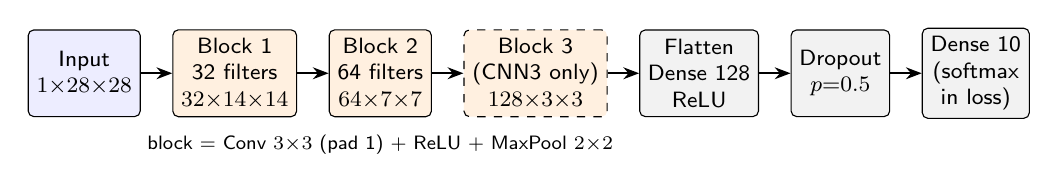
\begin{tikzpicture}[
  font=\sffamily\footnotesize,
  blk/.style={draw, rounded corners=2pt, align=center, minimum height=11mm, inner sep=3pt},
  inp/.style={blk, fill=blue!7},
  conv/.style={blk, fill=orange!12},
  dense/.style={blk, fill=gray!10},
  extra/.style={blk, fill=orange!12, dashed},
  arr/.style={-{Stealth[length=2mm]}, thick}
]
  \node[inp] (in) {Input\\$1{\times}28{\times}28$};
  \node[conv, right=4mm of in] (b1) {Block 1\\32 filters\\$32{\times}14{\times}14$};
  \node[conv, right=4mm of b1] (b2) {Block 2\\64 filters\\$64{\times}7{\times}7$};
  \node[extra, right=4mm of b2] (b3) {Block 3\\(CNN3 only)\\$128{\times}3{\times}3$};
  \node[dense, right=4mm of b3] (fc) {Flatten\\Dense 128\\ReLU};
  \node[dense, right=4mm of fc] (do) {Dropout\\$p{=}0.5$};
  \node[dense, right=4mm of do] (out) {Dense 10\\(softmax\\in loss)};
  \draw[arr] (in) -- (b1); \draw[arr] (b1) -- (b2); \draw[arr] (b2) -- (b3);
  \draw[arr] (b3) -- (fc); \draw[arr] (fc) -- (do); \draw[arr] (do) -- (out);
  \node[below=1mm of b2, font=\sffamily\scriptsize, align=center] {block = Conv $3{\times}3$ (pad 1) + ReLU + MaxPool $2{\times}2$};
\end{tikzpicture}}
\caption{Architecture. CNN2 skips the dashed block and flattens $64{\times}7{\times}7=3{,}136$ values; CNN3 flattens
$128{\times}3{\times}3=1{,}152$.}
\label{fig:arch}
\end{figure}

\begin{table}[t]
  \centering
  \caption{Architectures: Parameters, Compute and Receptive Field}
  \label{tab:arch}
  \setlength{\tabcolsep}{4pt}
  \begin{tabular}{@{}l r r r r@{}}
    \toprule
    & \multicolumn{2}{c}{Parameters} & & \\
    \cmidrule(lr){2-3}
    Layer & CNN2 & CNN3 & \multicolumn{2}{c}{MACs per image} \\
    \midrule
    Conv 1 ($1\to32$)            & 320       & 320       & \multicolumn{2}{r}{225{,}792} \\
    Conv 2 ($32\to64$)           & 18{,}496  & 18{,}496  & \multicolumn{2}{r}{3{,}612{,}672} \\
    Conv 3 ($64\to128$)          & ---       & 73{,}856  & \multicolumn{2}{r}{3{,}612{,}672\,(CNN3)} \\
    Dense ($\to128$)             & 401{,}536 & 147{,}584 & \multicolumn{2}{r}{401{,}408 / 147{,}456} \\
    Dense ($128\to10$)           & 1{,}290   & 1{,}290   & \multicolumn{2}{r}{1{,}280} \\
    \midrule
    \textbf{Total}               & \textbf{421{,}642} & \textbf{241{,}546} & \multicolumn{2}{r}{\textbf{4.24M / 7.60M}} \\
    Receptive field (px)         & $10\times10$ & $22\times22$ & & \\
    \bottomrule
  \end{tabular}
\end{table}

\subsection{Training}
Both networks are trained with identical settings (\cref{tab:train}), chosen as standard defaults rather than tuned:
there is no hyperparameter search. Training is deterministic: all random generators are seeded with 42,
deterministic kernels are enforced, and the function that trains a network also creates its starting weights and data
loaders, so its result cannot depend on anything run before it. A fresh-process retraining reproduces every reported
validation statistic exactly. Training runs on the CPU of an Apple M3 laptop with four threads, the same thread count
used for the classical models.

\begin{table}[t]
  \centering
  \caption{Training Configuration (Identical for Both Networks)}
  \label{tab:train}
  \begin{tabular}{@{}l l@{}}
    \toprule
    Loss & Cross-entropy (\cref{eq:ce}) \\
    Optimizer & Adam, $\eta=10^{-3}$, default $\beta_1,\beta_2,\epsilon$ \\
    Mini-batch & 64 (844 updates per epoch) \\
    Epochs & at most 30 \\
    Early stopping & on validation loss, patience 5, best weights restored \\
    Dropout & $p=0.5$ before the output layer \\
    Training data & 54{,}000 images (train split only) \\
    Seed / device & 42, deterministic / CPU, 4 threads \\
    \bottomrule
  \end{tabular}
\end{table}

\subsection{Selection and Evaluation Protocol}
\Cref{fig:protocol} summarizes the protocol. The rule for choosing between CNN2 and CNN3 was fixed before training:
higher validation accuracy, ties broken by fewer parameters. Only after the choice was recorded was each network
evaluated once on the test set by the same \texttt{evaluate()} function that scored every Phase~1 model: accuracy,
macro-F1, per-class precision and recall, the confusion matrix, model-only inference time per 1{,}000 images (best of
three runs) and model size (bytes of the serialized model). Each test evaluation is appended to an audit log, which ends
with exactly 14 rows: twelve classical experiments and two CNNs.

Phase~1 refit each classical model on all 60{,}000 training and validation images before testing. A CNN cannot be refit
in the same way, because the validation set is consumed during training by early stopping. The CNNs therefore learn from
10\% less data than the models they are compared with---a handicap that can only understate their advantage.

We report Wilson 95\% intervals~\cite{wilson1927probable} for test accuracy and compare classifiers with a two-sided
McNemar test with continuity correction on their paired test predictions~\cite{mcnemar1947note,dietterich1998approximate};
exact binomial $p$-values agree with the $\chi^2$ approximation in every case reported. All error analysis reads the
saved predictions; no model predicts on the test set a second time.

\begin{figure}[t]
\centering
\resizebox{\linewidth}{!}{%
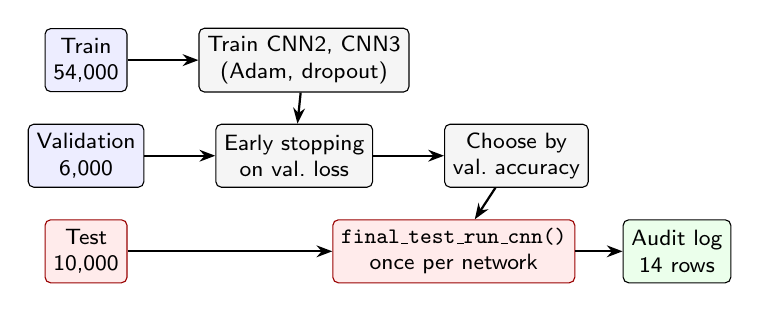
\begin{tikzpicture}[
  font=\sffamily\footnotesize,
  box/.style={draw, rounded corners=2pt, align=center, minimum height=8mm, inner sep=3pt},
  data/.style={box, fill=blue!7},
  proc/.style={box, fill=gray!8},
  lock/.style={box, fill=red!8, draw=red!60!black},
  arr/.style={-{Stealth[length=2mm]}, thick}
]
  \node[data] (tr)  {Train\\54{,}000};
  \node[data, below=4mm of tr] (va) {Validation\\6{,}000};
  \node[lock, below=4mm of va] (te) {Test\\10{,}000};

  \node[proc, right=9mm of tr] (fit) {Train CNN2, CNN3\\(Adam, dropout)};
  \node[proc, right=9mm of va] (es)  {Early stopping\\on val.\ loss};
  \node[proc, right=9mm of es] (sel) {Choose by\\val.\ accuracy};
  \node[lock, right=9mm of te, xshift=17mm] (once) {\texttt{final\_test\_run\_cnn()}\\once per network};
  \node[box, right=6mm of once, fill=green!8] (log) {Audit log\\14 rows};

  \draw[arr] (tr) -- (fit);
  \draw[arr] (fit) -- (es);
  \draw[arr] (va) -- (es);
  \draw[arr] (es) -- (sel);
  \draw[arr] (sel) -- (once);
  \draw[arr] (te) -- (once);
  \draw[arr] (once) -- (log);
\end{tikzpicture}}
\caption{Phase~2 protocol. Validation stops training and selects the network but never updates weights; the test set
(red) is read once per network, after selection, and each read is logged.}
\label{fig:protocol}
\end{figure}

% =====================================================================================
\section{Results}
\label{sec:results}

\subsection{Training Dynamics and Model Selection (RQ7)}
\Cref{fig:curves} shows both training runs and \cref{tab:val} the selection statistics. Validation loss bottoms out at
epoch~9 for CNN2 and epoch~12 for CNN3; afterwards training loss keeps falling (CNN3: 0.175\arrowc0.127) while
validation loss rises (0.193\arrowc0.208), the signature of overfitting, and early stopping ends each run five epochs
later and restores the best weights. At the selected epoch, training accuracy---measured with dropout active---lies
within 0.5\pp{} of validation accuracy, so the networks barely overfit. Early in training, validation accuracy
\emph{exceeds} training accuracy because the latter is averaged over an epoch of still-improving weights with dropout on.

Early stopping monitors loss, not accuracy, and the two can disagree: CNN2's validation accuracy kept rising to 0.9297 by
epoch~14 while its loss stayed above the epoch-9 minimum. Cross-entropy also penalizes over-confident mistakes, so it
deteriorates before accuracy does---the same mechanism that leaves modern networks poorly calibrated~\cite{guo2017calibration}.

\begin{figure}[t]
  \centering
  \includegraphics[width=\linewidth]{cnn_training_curves.png}
  \caption{Training and validation loss (top) and accuracy (bottom) per epoch. Dashed lines mark the epoch with the
  lowest validation loss, whose weights are kept.}
  \label{fig:curves}
\end{figure}

\begin{table}[t]
  \centering
  \caption{Validation Statistics Used for Model Selection}
  \label{tab:val}
  \setlength{\tabcolsep}{4pt}
  \begin{tabular}{@{}l c c c c r@{}}
    \toprule
    Network & Best / run & Val.\ loss & Val.\ acc. & Val.\ F1 & Train (s) \\
    \midrule
    CNN2 & 9 / 14  & 0.1976 & 0.9228 & 0.9223 & 198 \\
    \best{CNN3} & 12 / 17 & \best{0.1926} & \best{0.9308} & \best{0.9308} & 416 \\
    \midrule
    \multicolumn{3}{@{}l}{RBF SVM / HOG (Phase~1, 54k fit)} & 0.9157 & --- & --- \\
    \bottomrule
  \end{tabular}
\end{table}

By the pre-specified rule, \textbf{CNN3 is selected}. We do not read the 0.8\pp{} validation gap as evidence that depth
helps. A preliminary CNN2 run, identical except for the order of its mini-batches, reached 0.9320, and on the test set
the two networks disagree on 506 images with an almost even split (241 vs.\ 265; McNemar $p=0.31$). Run-to-run
variation of this size is well documented~\cite{bouthillier2021accounting}; a multi-seed study would be needed to
resolve a sub-point difference. What depth demonstrably buys is a 43\% smaller model.

\subsection{Test Performance (RQ5)}
\Cref{tab:test} places both networks next to the strongest classical models. CNN3 reaches \textbf{92.09\%} test accuracy
and \textbf{0.9208} macro-F1, and CNN2 91.85\% and 0.9176; both confidence intervals lie above the SVM's point estimate.
On the paired predictions, CNN3 corrects 417 images the SVM misclassifies and errs on 316 it gets right, a net 101
(\cref{tab:agree}); McNemar's test gives $\chi^2=13.6$, $p=2.2\times10^{-4}$. CNN2's advantage is also significant
($\chi^2=7.8$, $p=5.1\times10^{-3}$). \textbf{H1 is supported.} For both networks validation accuracy exceeds test
accuracy (by 0.99 and 0.43\pp), the selection bias expected when a model is chosen on the same
data~\cite{cawley2010overfitting}; the ranking is unchanged.

\begin{table*}[t]
  \centering
  \begin{threeparttable}
  \caption{Test Results of the CNNs and the Strongest Classical Models (Same Split, Same Evaluation Code)}
  \label{tab:test}
  \setlength{\tabcolsep}{5pt}
  \begin{tabular}{@{}l l c c c c c r r r@{}}
    \toprule
    Model & Input & Val.\ acc. & Test acc. & 95\% CI (\%) & Macro-F1 & Errors & Train (s) & Inference (ms/1k) & Size \\
    \midrule
    \best{CNN3} & Image & \best{0.9308} & \best{0.9209} & \best{91.54--92.60} & \best{0.9208} & \best{791} & 416 & 94.4 & 0.97\,MB \\
    CNN2        & Image & 0.9228 & 0.9185 & 91.30--92.37 & 0.9176 & 815 & 198 & 58.4 & 1.69\,MB \\
    \midrule
    RBF SVM     & HOG    & 0.9157 & 0.9108 & 90.51--91.62 & 0.9108 & 892   & 451 & 28{,}876.96\tnote{a} & 366.2\,MB \\
    RBF SVM     & Pixels & 0.9082 & 0.8970 & 89.09--90.28 & 0.8967 & 1{,}030 & 196 & 4{,}766.94 & 125.1\,MB \\
    Linear SVM  & HOG    & 0.8900 & 0.8898 & 88.35--89.58 & 0.8892 & 1{,}102 & 162 & 2.62\tnote{b} & 180.8\,KB \\
    \bottomrule
  \end{tabular}
  \begin{tablenotes}\footnotesize
    \item CNNs: trained on 54k, Apple M3 CPU, 4 threads. Classical models: refit on 60k, Apple M3 Pro, 4 workers
          (Phase~1~\cite{phase1report}). CI: Wilson 95\% interval. Inference: model-only time per 1{,}000 test images,
          best of three. Size: serialized model. Best result in bold.
    \item[a] Compares each image with 26{,}343 support vectors; treated as an upper bound in Phase~1. HOG extraction adds
          $\approx$216\,ms per 1{,}000 images to the HOG models.
    \item[b] Plus $\approx$216\,ms of HOG extraction end to end.
  \end{tablenotes}
  \end{threeparttable}
\end{table*}

\subsection{Cost (RQ8)}
The CNN is not only more accurate but far cheaper to run. CNN3 classifies 1{,}000 images in 94\,ms, against ${\approx}29.1$\,s
end to end for the RBF SVM on HOG, a ${\sim}300\times$ speed-up, from a 0.97\,MB model, ${\sim}377\times$ smaller than the
SVM's 366\,MB of stored support vectors. The SVM's cost grows with its training set because every prediction is
compared with each support vector; the CNN's is fixed by its architecture. Training costs are of the same order (minutes
on a laptop CPU). Within the CNNs, inference time tracks MACs rather than parameters: CNN3 is 43\% smaller but 62\% slower
than CNN2 (94 vs.\ 58\,ms), consistent with its 79\% higher MAC count (\cref{tab:arch}). Among the classical models, only
the Random Forest on pixels predicts faster (${\approx}12$\,ms per 1{,}000 images), at 4.5\pp{} lower accuracy and from a
366\,MB model; the 181\,KB Linear SVM on HOG is smaller but needs ${\approx}219$\,ms end to end once HOG extraction is
counted. The CNN therefore dominates the most accurate classical model on accuracy, latency and size simultaneously.

% =====================================================================================
\section{Error Analysis (RQ6)}
\label{sec:errors}

\textbf{Where the gain comes from.} \Cref{fig:recall} compares per-class recall. Relative to the SVM, CNN3 reduces errors
on T-shirt/top ($-22$), Pullover ($-28$), Coat ($-15$), Trouser ($-14$), Sneaker ($-14$) and Sandal ($-12$), and is slightly
worse on Dress ($+8$). On \textbf{Shirt it changes nothing}: recall is 75.1\% vs.\ 75.2\%, and Shirt\arrowc T-shirt/top
remains the largest confusion (110 vs.\ 104 images; \cref{fig:cm}). The CNN does label fewer non-shirts as Shirt (precision
77.4\% vs.\ 75.3\%), but it finds no more of the real ones.

\begin{figure*}[t]
  \centering
  \includegraphics[width=0.9\linewidth]{cnn_recall_vs_classical.png}
  \caption{Per-class test recall of the two CNNs and the best classical model. The CNNs improve every top except Shirt,
  where CNN3 equals the SVM and CNN2 is worse.}
  \label{fig:recall}
\end{figure*}

\begin{figure}[t]
  \centering
  \includegraphics[width=0.92\linewidth]{errors_confusion_cnn3_images.png}
  \caption{Row-normalized test confusion matrix of CNN3. The upper-body garments (T-shirt/top, Pullover, Coat, Shirt) form
  the dominant off-diagonal block, as they did for every Phase~1 model.}
  \label{fig:cm}
\end{figure}

\textbf{The two models trade shirts rather than fix them.} Of the 1{,}000 test shirts, 661 are classified correctly by
both models, 90 only by CNN3, 91 only by the SVM, and 158 by neither (McNemar $p=1.0$). Across all classes
(\cref{tab:agree}), the 101-image net gain is the difference of two large, nearly balanced
flows. Because the CNN removes easier errors first, the four upper-body classes hold a \emph{larger} share of what
remains: 539 of its 791 errors (68.1\%), against 573 of 892 (64.2\%) for the SVM. \textbf{H2 is rejected}: the gain is
real, but it does not arise chiefly where Phase~1 predicted, and the Shirt problem is untouched.

\begin{table}[t]
  \centering
  \caption{Agreement of CNN3 and the RBF SVM (HOG) on the 10{,}000 Test Images}
  \label{tab:agree}
  \begin{tabular}{@{}l c c r@{}}
    \toprule
    & \multicolumn{2}{c}{RBF SVM / HOG} & \\
    \cmidrule(lr){2-3}
    CNN3 & correct & wrong & Total \\
    \midrule
    correct & 8{,}792 & 417 & 9{,}209 \\
    wrong   & 316     & 475 & 791 \\
    \midrule
    Total   & 9{,}108 & 892 & 10{,}000 \\
    \bottomrule
  \end{tabular}
\end{table}

\textbf{Shared errors point to the data.} The 475 images that both models misclassify are revealing. The two models
share no features---one sees gradient histograms through a kernel, the other learned convolutional filters---yet on 398
of these images (83.8\%) they choose \emph{the same} wrong label, and 362 (76.2\%) are upper-body garments. Agreement
between independent models on a wrong answer is the signature of an ambiguous input or a questionable label rather than
of a model deficiency~\cite{northcutt2021pervasive}.

\textbf{Inspecting the mistakes.} \Cref{fig:mis} shows the first eight test shirts, in test-set order and not
hand-picked, that each model labels T-shirt/top. Most are short-sleeved and collarless; two in the CNN's grid
(test images \#612 and \#1129) are sleeveless tank tops. At $28\times28$, the cues that define a shirt---a collar, a button
placket, a cuff---occupy a handful of pixels when present at all, and for several of these images the label itself is
debatable. The grids also show the trade at the level of single images: CNN3 correctly identifies test \#40, whose
button placket is visible, and \#344 and \#628, all of which the SVM calls T-shirt/top, while the SVM correctly classifies
\#474, \#572, \#612, \#1056 and \#1129, which CNN3 calls T-shirt/top. Learned filters pick up some details that HOG misses,
and miss some that HOG's gradients capture.

\begin{figure}[t]
  \centering
  \includegraphics[width=\linewidth]{errors_misclassified_rbf_svm_hog_shirt_vs_t-shirt_top.png}\\[4pt]
  \includegraphics[width=\linewidth]{errors_misclassified_cnn3_images_shirt_vs_t-shirt_top.png}
  \caption{The first eight test images of class Shirt predicted as T-shirt/top by the RBF SVM on HOG (top, 8 of 104) and
  by CNN3 (bottom, 8 of 110). Several are collarless or sleeveless garments whose label is ambiguous at this resolution.}
  \label{fig:mis}
\end{figure}

% =====================================================================================
\section{Discussion}
\label{sec:discussion}
\textbf{Why did H2 fail?} The hypothesis assumed that the Shirt confusion was a \emph{representation} problem: that the
discriminative detail was present in the image and HOG failed to encode it. Three observations argue instead for an
\emph{information} problem. First, two representations with nothing in common fail on largely the same images, with the
same wrong label. Second, the CNN's improvement is broad---spanning footwear, trousers and the other tops---which is what a
generally better feature extractor produces, whereas a targeted fix would have concentrated on Shirt. Third, the failures
include garments that a human annotator could reasonably label either way. A larger network, augmentation or more data
can sharpen decision boundaries but cannot recover a collar that is two pixels wide or resolve a label that is genuinely
ambiguous; even far larger networks with augmentation stop at about 96\%~\cite{zhong2020random}, leaving several hundred
test errors. We therefore read our 92\% not as a modest CNN result, but as a sign that much of the
remaining error is already near the limit set by the data.

\textbf{Is a CNN worth it here?} For the catalog-tagging use case that motivated this project, yes: CNN3 is more
accurate, two orders of magnitude faster and smaller than the best classical model, and its cost does not grow with the
training set. Phase~1 found that the most practical classical choice was a 181\,KB Linear SVM on HOG at 88.98\%; CNN3
adds three points of accuracy and runs about twice as fast end to end, for a model that is still under 1\,MB. The classical pipeline's remaining advantage is simplicity:
it needs no deep-learning framework and its features are interpretable by construction.

\textbf{Threats to validity.}
\begin{itemize}
  \item \textbf{Single training run per network.} Seed variance was not measured systematically; the one available
        repetition (CNN2, 0.9228 vs.\ 0.9320 on validation) suggests about 1\pp. The CNN-vs-SVM conclusion is supported by
        a paired test on 10{,}000 images; the CNN3-vs-CNN2 comparison is explicitly inconclusive.
  \item \textbf{Unequal training data.} The CNNs saw 54k images, the classical models 60k; this biases the comparison
        against the CNN.
  \item \textbf{Fixed hyperparameters.} No learning-rate, width or dropout search was run, and augmentation and batch
        normalization were excluded by design. The CNN result is therefore a lower bound on what this model family
        achieves.
  \item \textbf{Timing hardware.} CNN timings come from an Apple M3, classical timings from an Apple M3 Pro; only the
        two-order-of-magnitude gaps should be read as firm.
  \item \textbf{Label quality.} Our evidence of ambiguous labels is qualitative; we did not relabel any images, so all
        accuracies are measured against the official labels.
\end{itemize}

% =====================================================================================
\section{Conclusion and Future Work}
\label{sec:conclusion}
Under a protocol that holds the data, the test set and the evaluation code fixed, a three-block CNN with fewer than a
quarter of a million parameters outperforms the best of twelve tuned classical pipelines on Fashion-MNIST: 92.09\% vs.\
91.08\% test accuracy, a statistically significant 101 fewer errors, at roughly 1/300 of the inference time and 1/377 of
the size. The hypothesis that it would win \emph{by fixing the shirts} is rejected. The gain is spread across many
classes, Shirt recall is unchanged, and the errors that remain are shared with a model that sees the image completely
differently---evidence that the limiting factor is the resolution and labeling of the data, not the choice between
handcrafted and learned features. A third convolutional block makes the network smaller, but its accuracy benefit
cannot be distinguished from run-to-run variation.

\textbf{Future work.} (i)~Repeat training over several seeds to bound variance and settle the depth comparison.
(ii)~Use the trained CNN as a feature extractor for the Phase~1 RBF SVM~\cite{razavian2014cnn}, holding the classifier
fixed to isolate the contribution of the representation. (iii)~Audit the shared errors with a confident-learning
procedure~\cite{northcutt2021pervasive} to estimate how much of the residual error is label noise. (iv)~Test whether
augmentation or higher-resolution inputs change the Shirt result, which would distinguish a capacity limit from an
information limit.

\textbf{Reproducibility.} Code, the committed split, all result files, per-epoch training histories, figures, the
test-set audit log and a decision log recording the reason for every choice are available at
\url{https://github.com/rajdeep-2004/fashion-image-classification-benchmark} (release \texttt{v1.0.0} for Phase~1).
Training is seeded and deterministic on CPU; a fresh clone regenerates every reported number.

% =====================================================================================
\begin{thebibliography}{99}

\bibitem{lecun2015deep}
Y.~LeCun, Y.~Bengio, and G.~Hinton, ``Deep learning,'' \emph{Nature}, vol.~521, no.~7553, pp.~436--444, 2015.

\bibitem{krizhevsky2012imagenet}
A.~Krizhevsky, I.~Sutskever, and G.~E. Hinton, ``ImageNet classification with deep convolutional neural networks,'' in
\emph{Adv. Neural Inf. Process. Syst. (NeurIPS)}, vol.~25, 2012, pp.~1097--1105.

\bibitem{simonyan2015very}
K.~Simonyan and A.~Zisserman, ``Very deep convolutional networks for large-scale image recognition,'' in \emph{Proc.
Int. Conf. Learn. Represent. (ICLR)}, 2015.

\bibitem{he2016deep}
K.~He, X.~Zhang, S.~Ren, and J.~Sun, ``Deep residual learning for image recognition,'' in \emph{Proc. IEEE Conf.
Comput. Vis. Pattern Recognit. (CVPR)}, 2016, pp.~770--778.

\bibitem{kaufman2012leakage}
S.~Kaufman, S.~Rosset, C.~Perlich, and O.~Stitelman, ``Leakage in data mining: Formulation, detection, and avoidance,''
\emph{ACM Trans. Knowl. Discov. Data}, vol.~6, no.~4, pp.~1--21, 2012.

\bibitem{cawley2010overfitting}
G.~C.~Cawley and N.~L.~C.~Talbot, ``On over-fitting in model selection and subsequent selection bias in performance
evaluation,'' \emph{J. Mach. Learn. Res.}, vol.~11, pp.~2079--2107, 2010.

\bibitem{bouthillier2021accounting}
X.~Bouthillier \emph{et al.}, ``Accounting for variance in machine learning benchmarks,'' in \emph{Proc. Mach. Learn.
Syst. (MLSys)}, 2021.

\bibitem{phase1report}
T.~Singh, A.~Mishra, R.~Sanyal, R.~Srivastav, and O.~Nagre, ``How far can classical machine learning go on
Fashion-MNIST? A leak-free benchmark of raw pixels vs.\ HOG features, with cost and error analysis,'' Capstone Project
Report, Phase~1, Newton School of Technology, Rishihood University, 2026.

\bibitem{xiao2017fashion}
H.~Xiao, K.~Rasul, and R.~Vollgraf, ``Fashion-MNIST: A novel image dataset for benchmarking machine learning
algorithms,'' \emph{arXiv preprint arXiv:1708.07747}, 2017.

\bibitem{dalal2005histograms}
N.~Dalal and B.~Triggs, ``Histograms of oriented gradients for human detection,'' in \emph{Proc. IEEE Conf. Comput.
Vis. Pattern Recognit. (CVPR)}, 2005, pp.~886--893.

\bibitem{cortes1995support}
C.~Cortes and V.~Vapnik, ``Support-vector networks,'' \emph{Mach. Learn.}, vol.~20, no.~3, pp.~273--297, 1995.

\bibitem{hubel1962receptive}
D.~H. Hubel and T.~N. Wiesel, ``Receptive fields, binocular interaction and functional architecture in the cat's visual
cortex,'' \emph{J. Physiol.}, vol.~160, no.~1, pp.~106--154, 1962.

\bibitem{fukushima1980neocognitron}
K.~Fukushima, ``Neocognitron: A self-organizing neural network model for a mechanism of pattern recognition unaffected
by shift in position,'' \emph{Biol. Cybern.}, vol.~36, no.~4, pp.~193--202, 1980.

\bibitem{rumelhart1986learning}
D.~E. Rumelhart, G.~E. Hinton, and R.~J. Williams, ``Learning representations by back-propagating errors,''
\emph{Nature}, vol.~323, no.~6088, pp.~533--536, 1986.

\bibitem{lecun1989backpropagation}
Y.~LeCun \emph{et al.}, ``Backpropagation applied to handwritten zip code recognition,'' \emph{Neural Comput.}, vol.~1,
no.~4, pp.~541--551, 1989.

\bibitem{lecun1998gradient}
Y.~LeCun, L.~Bottou, Y.~Bengio, and P.~Haffner, ``Gradient-based learning applied to document recognition,''
\emph{Proc. IEEE}, vol.~86, no.~11, pp.~2278--2324, 1998.

\bibitem{nair2010rectified}
V.~Nair and G.~E. Hinton, ``Rectified linear units improve restricted Boltzmann machines,'' in \emph{Proc. Int. Conf.
Mach. Learn. (ICML)}, 2010, pp.~807--814.

\bibitem{goodfellow2016deep}
I.~Goodfellow, Y.~Bengio, and A.~Courville, \emph{Deep Learning}. Cambridge, MA, USA: MIT Press, 2016.

\bibitem{zeiler2014visualizing}
M.~D. Zeiler and R.~Fergus, ``Visualizing and understanding convolutional networks,'' in \emph{Proc. Eur. Conf. Comput.
Vis. (ECCV)}, 2014, pp.~818--833.

\bibitem{razavian2014cnn}
A.~S. Razavian, H.~Azizpour, J.~Sullivan, and S.~Carlsson, ``CNN features off-the-shelf: An astounding baseline for
recognition,'' in \emph{Proc. IEEE Conf. Comput. Vis. Pattern Recognit. Workshops (CVPRW)}, 2014, pp.~806--813.

\bibitem{srivastava2014dropout}
N.~Srivastava, G.~Hinton, A.~Krizhevsky, I.~Sutskever, and R.~Salakhutdinov, ``Dropout: A simple way to prevent neural
networks from overfitting,'' \emph{J. Mach. Learn. Res.}, vol.~15, pp.~1929--1958, 2014.

\bibitem{prechelt1998early}
L.~Prechelt, ``Early stopping---but when?'' in \emph{Neural Networks: Tricks of the Trade}, ser. Lecture Notes in
Computer Science, vol.~1524. Berlin, Germany: Springer, 1998, pp.~55--69.

\bibitem{kingma2015adam}
D.~P. Kingma and J.~Ba, ``Adam: A method for stochastic optimization,'' in \emph{Proc. Int. Conf. Learn. Represent.
(ICLR)}, 2015.

\bibitem{ioffe2015batch}
S.~Ioffe and C.~Szegedy, ``Batch normalization: Accelerating deep network training by reducing internal covariate
shift,'' in \emph{Proc. Int. Conf. Mach. Learn. (ICML)}, 2015, pp.~448--456.

\bibitem{zagoruyko2016wide}
S.~Zagoruyko and N.~Komodakis, ``Wide residual networks,'' in \emph{Proc. Brit. Mach. Vis. Conf. (BMVC)}, 2016.

\bibitem{zhong2020random}
Z.~Zhong, L.~Zheng, G.~Kang, S.~Li, and Y.~Yang, ``Random erasing data augmentation,'' in \emph{Proc. AAAI Conf. Artif.
Intell.}, vol.~34, no.~7, 2020, pp.~13001--13008.

\bibitem{mcnemar1947note}
Q.~McNemar, ``Note on the sampling error of the difference between correlated proportions or percentages,''
\emph{Psychometrika}, vol.~12, no.~2, pp.~153--157, 1947.

\bibitem{dietterich1998approximate}
T.~G. Dietterich, ``Approximate statistical tests for comparing supervised classification learning algorithms,''
\emph{Neural Comput.}, vol.~10, no.~7, pp.~1895--1923, 1998.

\bibitem{northcutt2021pervasive}
C.~G. Northcutt, A.~Athalye, and J.~Mueller, ``Pervasive label errors in test sets destabilize machine learning
benchmarks,'' in \emph{Proc. NeurIPS Datasets and Benchmarks Track}, 2021.

\bibitem{wilson1927probable}
E.~B. Wilson, ``Probable inference, the law of succession, and statistical inference,'' \emph{J. Amer. Statist.
Assoc.}, vol.~22, no.~158, pp.~209--212, 1927.

\bibitem{guo2017calibration}
C.~Guo, G.~Pleiss, Y.~Sun, and K.~Q. Weinberger, ``On calibration of modern neural networks,'' in \emph{Proc. Int.
Conf. Mach. Learn. (ICML)}, 2017, pp.~1321--1330.

\end{thebibliography}

\end{document}
